\section{Excitons at finite momentum}\label{sec:10.5}

At a momentum transfer equal to the valley momentum $\vect{k}_{\mathrm{c}}$, the lowest final state of silicon is not a free electron and hole at the indirect gap of \SI{1.17}{eV}. It is the pair bound by its own attraction, \SI{14.7}{meV} lower (\cref{sec:4.9}), and for the density coupling of \cref{sec:10.2} this attraction is the first correction beyond the random-phase approximation with local fields. Whether a given coupling can reach the bound pair is a question of symmetry. Besides adding a line below the threshold, the attraction raises the probability of finding the electron at the hole in every pair of the continuum. The continuum just above $E_{\mathrm{min}}(\vect{q})$ grows at the expense of higher energies, and the change is largest in the first eV above the gap, where most of the rate of light dark matter lies. \Cref{sec:10.2} wrote the screened rate as an integral of the loss function, and \cref{sec:4.9} gave the loss function of the Bethe--Salpeter equation. Put together at finite $\vect{q}$, they give the rate as a sum over exciton lines. We will find where its onset lies, which lines a density coupling can reach at the zone boundary of silicon, and how much a resonant-only solution of the equation costs. The spin-triplet excitons, which only spin couplings reach, close the section.

\subsection{The exciton rate}\label{sec:10.5-rate}

The rate of \cref{eq:10.2-rate} holds for any loss function, so the electron--hole attraction enters it through $L$ alone. With the eigenpairs $E_\lambda(\vect{q})$ and $A^\lambda_{cv\vect{k}}(\vect{q})$ of \cref{eq:4.9-bse} the structure factor is \cref{eq:4.9-S}, a sum of lines, one per exciton. Each line carries the squared matrix element of the density between the ground state and the singlet exciton $\lambda$. The singlet pair state $cv\vect{k}$ has amplitude $\sqrt{g_{\mathrm{deg}}}\,\rho_{cv}(\vect{k},\vect{q})$ to be created by $n_e(\vect{q})$, and the exciton is the superposition $\sum_{cv\vect{k}}A^\lambda_{cv\vect{k}}|cv\vect{k}\rangle$, so $\langle\lambda|n_e(\vect{q})|0\rangle = \sqrt{g_{\mathrm{deg}}}\,\rho_{\lambda0}(\vect{q})$ with
\begin{equation}
  \rho_{\lambda0}(\vect{q}) = \sum_{cv\vect{k}}A^\lambda_{cv\vect{k}}(\vect{q})^*\,\rho_{cv}(\vect{k},\vect{q}) ,
  \label{eq:10.5-formfactor}
\end{equation}
the exciton form factor. It is the coherent sum of \cref{sec:4.9}: the vertices of all the transitions in the exciton add with the amplitudes of its envelope. At $T = 0$ and $\omega > 0$, $L = (e^2/2q^2)S$ by \cref{eq:4.4-SL}, and \cref{eq:4.9-S} gives $L = (4\pi^2\alpha g_{\mathrm{deg}}/Vq^2)\sum_\lambda|\rho_{\lambda0}|^2\delta(\omega - E_\lambda)/|\varepsilon_{\mathrm{mac}}|^2$. In \cref{eq:10.2-rate} the factor $4\pi^2\alpha$ cancels against $8\pi^2\alpha$ and $q^3/q^2$ leaves one power of $q$.
\begin{keyresult}[Exciton rate at finite momentum]
\begin{equation}
  \frac{\dd\mathcal{R}}{\dd\omega} = \frac{\rho_\chi\,\sigmae\,g_{\mathrm{deg}}}{2\rho_T\,\mchi\,\mu_{\chi e}^2}\int\dd q\;q\,\eta\bigl(\vmin(q,\omega)\bigr)\,\FDM(q)^2\,\biggl\langle\frac1\Vol\sum_\lambda\frac{|\rho_{\lambda0}(\vect{q})|^2}{|\varepsilon_{\mathrm{mac}}(\vect{q},\omega)|^2}\,\delta\bigl(\omega - E_\lambda(\vect{q})\bigr)\biggr\rangle_{\hat{\vect{q}}} ,
  \label{eq:10.5-rate}
\end{equation}
with $\langle\cdots\rangle_{\hat{\vect{q}}}$ the average over the directions of $\vect{q}$, the exciton energies and form factors of \cref{eq:4.9-bse,eq:10.5-formfactor} at the momentum transfer $\vect{q}$ (reduced to the first zone in the kernels, \cref{sec:4.9}), and $g_{\mathrm{deg}} = 2$.
\end{keyresult}
\noindent Without the kernels each $\lambda$ is one transition, $\rho_{\lambda0} = \rho_{cv}$, $E_\lambda = \varepsilon_{c,\vect{k}+\vect{q}} - \varepsilon_{v\vect{k}}$, and \cref{eq:10.5-rate} is the random-phase rate of \cref{sec:10.2}; without $1/|\varepsilon_{\mathrm{mac}}|^2$ as well, it is the crystal form-factor rate of \cref{sec:10.1}. With the attraction on, the energies $E_\lambda(\vect{q})$ start below $E_{\mathrm{min}}(\vect{q})$, so the support of the spectrum moves down, and the weights $|\rho_{\lambda0}|^2$ are coherent sums, so the spectrum changes shape at fixed total weight. The $f$-sum rule of \cref{sec:4.3} holds for the exact $L$ at every $\vect{q}$, and what the attraction adds at low energy it removes higher up. For a rate this redistribution is not neutral: $\eta(\vmin)$ falls with $\omega$ at fixed $q$, and a particle that cannot deposit more than $\tfrac12\mchi v_{\mathrm{max}}^2$ sees only the low side. The line form with $|\varepsilon_{\mathrm{mac}}|^2$ in the denominator holds when no single line changes $\varepsilon_{\mathrm{mac}}$ near its own energy, which at keV momentum transfers, where the Coulomb factor $e^2/q^2$ is small, is always the case (\cref{sec:4.9}).

The equation is solved as in \cref{sec:4.9}, now at the reduced momentum $\vect{q}_r$ of each $\vect{q}$. It needs pairs from $(v,\vect{k})$ to $(c,\vect{k}+\vect{q}_r)$ on a grid of crystal momenta, quasiparticle energies or a scissor on Kohn--Sham bands, the screened interaction $W^{\mathrm{scr}}$ for all grid differences, and the head of the exchange kernel at the unreduced $\vect{G}_q$ left out (\cref{app:E.6}). The first such calculations for dark matter were made for GaAs and NaI, with the scissor set to the measured gaps, a $6^3$ grid, 10 conduction bands and momenta along [100] up to \SI{14.7}{keV}~\cite{taufertshofer2026excitonic}. In both materials the loss function with the attraction lies above the random-phase one with local fields at low energy, at all the momenta shown. In GaAs the rate changes little. In NaI, whose lowest optical exciton lies about \SI{0.3}{eV} below the gap (an absorption peak at \SI{5.6}{eV} against a gap of \SI{5.9}{eV}~\cite{taufertshofer2026excitonic}), some seventy times deeper than the \SI{4.2}{meV} of GaAs (\cref{sec:4.9}), the rate at energies near the gap rises enough to improve the projected reach above a few MeV by close to an order of magnitude~\cite{taufertshofer2026excitonic}. No such calculation exists yet for silicon or germanium. \Cref{app:E.15} specifies one, with the coupling between pair creation and annihilation that the published calculations drop, and with the bound lines added from the effective-mass model below, since a $6^3$ or even a $24^3$ grid cannot resolve an exciton of radius \SI{4.2}{nm}.

What the attraction does at a dark-matter momentum transfer can be seen in silicon itself, in the model of \cref{fig:4-bse} carried to finite $\vect{q}$ (\cref{fig:10-xq}). At $|\vect{q}| = \SI{0.91}{keV}$ along [100], halfway to the valley, the lowest pair of the model costs \SI{1.69}{eV}. The attraction changes the proper absorption $\varepsilon_2$ the way it did at $q \to 0$. The main peak moves from \SI{5.3}{eV} to \SI{4.5}{eV} and grows from 16.5 to 27.5. The weight below \SI{3}{eV} grows by a factor of 2.2 over the random-phase value with local fields. The loss function follows with the screening of the same model, whose static value rises from 6.56 to 7.80. Between the onset and \SI{3.5}{eV} the attraction raises $L$ by a nearly constant 27 to 29 percent, by 49 percent at \SI{4}{eV}, and by about 30 percent above. The rise at high energies is partly an artifact: four conduction bands and the Tamm--Dancoff form do not hold the $f$-sum fixed, and the first moment of $\varepsilon_2$ below \SI{10}{eV} falls by 12 percent. The grid, ten points per direction, resolves no bound line, and the lines of \cref{sec:10.5-lines} lie below the gray region of the figure. For a rate the near-edge factor is what counts. Dark matter below a few MeV reaches only the first two eV above $E_{\mathrm{min}}(\vect{q})$, and there the attraction adds about a quarter to the screened loss function, on top of whatever bound lines the grid misses.

\begin{figure}[tbp]
  \centering
  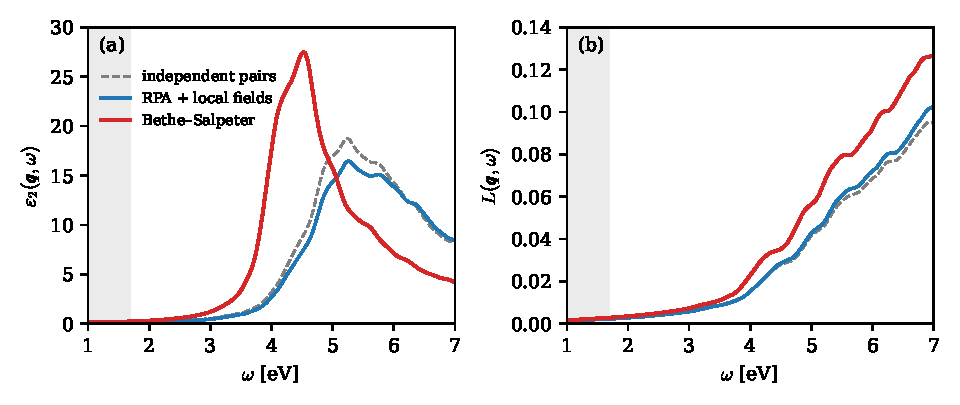
\includegraphics[width=\linewidth]{figures/ch10/fig10_4.pdf}
  \caption{The electron--hole attraction at finite momentum transfer in silicon, in a model calculation: $|\vect{q}| = \SI{0.91}{keV}$ ($0.4\times2\pi/a$) along [100]. States from the empirical pseudopotential of Cohen and Bergstresser~\cite{cohen1966band}, fitted to measured transition energies (model indirect gap \SI{0.82}{eV}; no scissor); 4 valence and 4 conduction bands on a shifted $10^3$ grid over the full zone (16{,}000 pairs); the 59 shortest reciprocal vectors in both kernels; direct kernel with the model dielectric function of Cappellini and coworkers~\cite{cappellini1993model} with $\varepsilon_\infty = 11.7$; Tamm--Dancoff resonant block with both time orderings, \cref{eq:4.9-epsmac}; Lorentzian broadening \SI{0.15}{eV}. On this grid the independent-pair spectrum agrees with a $15^3$ grid within 8 percent below \SI{6}{eV}. Gray: below the lowest pair of the grid, \SI{1.69}{eV}, where the curves are broadening tails; the bound lines are not resolved. Dashed: independent pairs (with the head screening only, in panel b); blue: random-phase approximation with local fields; red: Bethe--Salpeter equation. (a) Proper absorption $\varepsilon_2(\vect{q},\omega)$. (b) Loss function. The fitted bands already contain part of the excitonic shift, which the attraction then counts again (\cref{sec:4.9}).}
  \label{fig:10-xq}
\end{figure}

\subsection{Elliott onset and bound exciton lines}\label{sec:10.5-lines}

Near the bottom of the pair continuum at a given $\vect{q}$ the exciton form factor has a closed form, and with it the onset of \cref{eq:10.5-rate}. At fixed $\vect{q}$ the pair energy $\varepsilon_{c,\vect{k}+\vect{q}} - \varepsilon_{v\vect{k}}$ has its minimum $E_{\mathrm{min}}(\vect{q})$ of \cref{eq:3.3-Emin} at some $\vect{k}_0(\vect{q})$, and near it the pair energy rises quadratically in $\vect{k} - \vect{k}_0$, with a reduced mass set by the curvatures of the two bands at $\vect{k}_0$ and $\vect{k}_0 + \vect{q}$. This is the situation of \cref{eq:4.9-dispersion}, with the extremum of the pair energy in place of the band extrema. The relative motion obeys the hydrogenic equation \cref{eq:4.9-envelope}, and the bound states sit at $E_{\mathrm{min}}(\vect{q}) - E_x^b/n^2$. In silicon at $\vect{q} = \vect{k}_{\mathrm{c}}$ the pair minimum joins the two band extrema and $E_x^b$ is the measured \SI{14.7}{meV}. Away from the valley, $\vect{k}_0$ moves off the band extrema, the reduced mass changes, and $E_x^b$ with it (\cref{eq:E.15-disp}); we keep the symbols $E_x^b$, $a_x$ and $\mu_x$ for the values at the $\vect{q}$ in question.

When $\rho_{cv}(\vect{k},\vect{q})$ is smooth and nonzero at $\vect{k}_0$, the Elliott form \cref{eq:4.9-elliott} applies: $|\rho_{\lambda0}|^2 = \Vol|F_\lambda(0)|^2|\rho_{cv}(\vect{k}_0,\vect{q})|^2$. For the bound $s$ states, $|F_{ns}(0)|^2 = 1/(\pi a_x^3n^3)$. For the unbound states of relative momentum $\kappa$, normalized in the volume $\Vol$, $\Vol|F_{\kappa}(0)|^2$ is its free value, one, times the factor by which the attraction raises the probability of finding the electron at the hole. That factor is the Fermi factor \cref{eq:2.2-fermi} of an electron leaving a charge, with the coupling $\alpha/\varepsilon_\infty$ and the mass $\mu_x$ in place of $\alpha$ and $m_e$, so that $\xi_{\mathrm{C}} = 1/(\kappa a_x)$. With $\kappa^2 = 2\mu_x(\omega - E_{\mathrm{min}})$ and $2\mu_xE_x^ba_x^2 = 1$ from \cref{eq:4.9-WM}, the line sum in \cref{eq:10.5-rate} becomes
\begin{equation}
  \begin{aligned}
  \frac1\Vol\sum_\lambda|\rho_{\lambda0}|^2\delta(\omega - E_\lambda) = |\rho_{cv}(\vect{k}_0,\vect{q})|^2\biggl[&\sum_{n\ge1}\frac{\delta\bigl(\omega - E_{\mathrm{min}} + E_x^b/n^2\bigr)}{\pi a_x^3n^3} \\
  &+ \Theta(\omega - E_{\mathrm{min}})\,\frac{(2\mu_x)^{3/2}(\omega - E_{\mathrm{min}})^{1/2}}{4\pi^2}\,\frac{2\pi\xi_{\mathrm{C}}}{1 - \ee^{-2\pi\xi_{\mathrm{C}}}}\biggr] ,
  \end{aligned}
  \label{eq:10.5-lines}
\end{equation}
with $\xi_{\mathrm{C}} = [E_x^b/(\omega - E_{\mathrm{min}})]^{1/2}$. The density of free pairs, $\int\dd^3\kappa\,(2\pi)^{-3}\delta(\omega - E_{\mathrm{min}} - \kappa^2/2\mu_x)$, supplies the square root. The two parts meet smoothly. The lines crowd toward $E_{\mathrm{min}}$ with spacing $2E_x^b/n^3$, so their weight per unit energy tends to $1/(2\pi a_x^3E_x^b)$, and as $\omega \to E_{\mathrm{min}}^+$ the continuum tends to $(2\mu_x)^{3/2}(E_x^b)^{1/2}/2\pi$, which is the same number. The edge of the excitonic spectrum at fixed $\vect{q}$ is therefore a series of lines followed by a finite step, where independent pairs start from zero as $(\omega - E_{\mathrm{min}})^{1/2}$.

How much weight the lines take is a short calculation. Their total is $\sum_n 1/(\pi a_x^3n^3) = \zeta(3)/(\pi a_x^3)$. The free continuum without the Fermi factor holds $(2\mu_x)^{3/2}\epsilon^{3/2}/6\pi^2$ between $E_{\mathrm{min}}$ and $E_{\mathrm{min}} + \epsilon$. With $(2\mu_x)^{3/2} = 1/(a_x^3(E_x^b)^{3/2})$ the two are equal at $\epsilon = (6\pi\zeta(3))^{2/3}E_x^b = 8.0\,E_x^b$: the bound lines together carry as much weight as the free pairs within eight binding energies of the edge would have carried. The attraction does not stop there. Above the edge the Fermi factor is $6.3$ at $\omega - E_{\mathrm{min}} = E_x^b$, falls to 2.3 at $10\,E_x^b$, and is still $1 + \pi\xi_{\mathrm{C}} + \dots$ far above, a slow approach to one. The hydrogenic form of that tail is not to be trusted beyond a few tenths of an eV, where the bands stop being parabolic and the pair samples the screening at shorter distances, and the sign is all it fixes there. The spectrum it describes comes from the region near the pair minimum only. In silicon at $\vect{q} = \vect{k}_{\mathrm{c}}$ the heavy and light holes at the valence maximum each add their own copy of \cref{eq:10.5-lines}, with their own masses and vertices.

\begin{workedexample}{The exciton line of silicon below the pair onset}\label{we:10-xline}
Take a momentum transfer close to $\vect{k}_{\mathrm{c}}$ in silicon, where $E_{\mathrm{min}}$ is the gap. With the low-temperature gap of \SI{1.17}{eV} and $E_x^b = \SI{14.7}{meV}$, the $1s$ line sits at \SI{1.155}{eV} and the $2s$ line at $\SI{1.17}{eV} - E_x^b/4 = \SI{1.166}{eV}$; the radius is $a_x = \SI{4.2}{nm}$ (\cref{sec:4.9}). For a vertex that is smooth at the band extrema, \cref{eq:10.5-lines} gives the $1s$ line the weight $|\rho_{cv}|^2/(\pi a_x^3) = |\rho_{cv}|^2\times\SI{4.3e-6}{\angstrom^{-3}}$ per unit volume. It is $1/\zeta(3) = 0.83$ of all the lines, and it equals the free-pair weight within $(6\pi)^{2/3}E_x^b = 7.1\,E_x^b = \SI{0.10}{eV}$ of the edge. A particle that deposits $\omega$ between \SI{1.155}{eV} and \SI{1.17}{eV} at this $\vect{q}$ has no free pair to make and makes the exciton; one that deposits \SI{1.27}{eV} finds the free-pair density raised by the factor $2.6$. For the rate integrated over $\omega$, a line \SI{14.7}{meV} below the edge changes little; for the threshold mass it changes even less. The kinematic floor of \cref{eq:1.3-mmin}, $2\Eg/v_{\mathrm{max}}^2 = \SI{0.333}{MeV}$, becomes $2(\Eg - E_x^b)/v_{\mathrm{max}}^2 = \SI{0.329}{MeV}$, a shift of 1.3 percent, and \cref{sec:3.3} showed that this floor is not reached at all, since the momentum at which a particle that light deposits most energy falls short of the valley. Where the zero-phonon edge of silicon lies, and that its first line is weak, are the subjects of \cref{sec:13.1,sec:13.9}. The line is weak because on the valley axis the vertex at the extrema vanishes, and the $1s$ line is dark.
\end{workedexample}

\subsection{Selection rules at the zone boundary}\label{sec:10.5-rules}

Spin decides first which excitons a dark-matter coupling can make in silicon. The ground state is a singlet, the density does not act on spin, and $n_e(\vect{q})$ creates only singlet excitons, the ones of \cref{eq:4.9-bse} with $g_{\mathrm{deg}}K^{\mathrm{x}}$. The triplets, in which the electron and hole spins combine to one, are reached by the spin density and the spin current of \cref{tab:10-minimal}, and \cref{sec:10.5-triplet} treats them. Crystal momentum decides next. The lowest exciton of silicon has the electron in a valley and the hole at $\mathrm{\Gamma}$, so it carries $\vect{k}_{\mathrm{c}}$ up to a reciprocal-lattice vector, and a coupling reaches it at first order only through $\vect{q} = \vect{k}_{\mathrm{c}} + \vect{G}$. Light, with $q \approx 0$, needs a phonon (\cref{sec:6.5}). Dark matter of a few hundred keV and more carries $|\vect{k}_{\mathrm{c}}| = \SI{1.94}{keV}$ and needs none.

The symmetry of the states at the extrema decides last, and it is what makes the first line of silicon weak. Take $\vect{q} = \vect{k}_{\mathrm{c}}$ along [100], the $x$ axis, with no Umklapp vector. Consider the operations of the cubic group that leave this axis fixed: the rotations by multiples of $90^\circ$ about it and the mirrors that contain it. The conduction state at the valley minimum is invariant under all of them, and so is the operator $\ee^{\ii\vect{q}\cdot\vect{r}}$. The three valence states at the maximum transform like the products $yz$, $zx$ and $xy$ (in the notation of the band structure, $\mathrm{\Gamma}_{25'}$). Under the quarter turn about $x$, which takes $y \to z$ and $z \to -y$, $yz$ changes sign. The pair $(zx, xy)$ transforms like the two components $(z, y)$ of a vector across the axis and contains no invariant combination. A matrix element $\langle c,\vect{k}_{\mathrm{c}}|\ee^{\ii\vect{q}\cdot\vect{r}}|v,\mathrm{\Gamma}\rangle$ between an invariant state, through an invariant operator, to a state with no invariant part vanishes. Half of these operations carry the fractional translation of the diamond structure (\cref{app:C.17}), which multiplies the Bloch states and the operator by phases; for $\vect{q} = \vect{k}_{\mathrm{c}}$ exactly, the phase of the operator, $\ee^{-\ii\vect{q}\cdot\vect{\tau}_2}$, cancels that of the conduction state, $\ee^{-\ii\vect{k}_{\mathrm{c}}\cdot\vect{\tau}_2}$, and the argument stands. In germanium the valleys lie along [111]. The rotations by $120^\circ$ about that axis and the mirrors containing it leave the combination $yz + zx + xy$ invariant, and the vertex at the extrema does not vanish.

A vertex that vanishes at the extrema grows linearly away from them: $\rho_{cv}(\vect{k},\vect{q}) \simeq (\vect{k} - \vect{k}_0)\cdot\vect{g}$ with $\vect{g} = \nabla_{\vect{k}}\rho_{cv}$, and $\vect{q}$ itself off the axis adds a term proportional to its distance $\delta q_\perp$ from it. Transitions with a vertex of this kind are called second class~\cite{elliott1957intensity}. Their exciton form factor picks out the gradient of the envelope where the electron meets the hole. From $A_{\vect{k}} = \Vol^{-1/2}\int\dd^3r\,F(\vect{r})\ee^{-\ii\vect{k}\cdot\vect{r}}$, $\sum_{\vect{k}}A_{\vect{k}}\,\vect{k}\cdot\vect{g} = -\ii \Vol^{1/2}\,\vect{g}\cdot\nabla F(0)$, which vanishes for $s$ states and is nonzero for the $p$ state oriented along $\vect{g}$. Its envelope is $R_{n1}(r)\,(3/4\pi)^{1/2}\cos\theta$, with $\theta$ measured from $\vect{g}$, and the hydrogen radial function starts as $R_{n1} \to \tfrac23[(n^2 - 1)/n^5]^{1/2}r/a_x^{5/2}$; for $n = 2$ this is $R_{21} = r\,\ee^{-r/2a_x}/(2\sqrt6\,a_x^{5/2})$. So $|\vect{g}\cdot\nabla F_{np}(0)|^2 = |\vect{g}|^2(n^2 - 1)/(3\pi a_x^5n^5)$, and in place of the $s$ lines of \cref{eq:10.5-lines},
\begin{equation}
  \frac1\Vol\sum_{\lambda\in\text{lines}}|\rho_{\lambda0}|^2\delta(\omega - E_\lambda) = |\nabla_{\vect{k}}\rho_{cv}|^2\sum_{n\ge2}\frac{n^2 - 1}{3\pi a_x^5n^5}\,\delta\bigl(\omega - E_{\mathrm{min}} + E_x^b/n^2\bigr) \qquad\text{(second class)} .
  \label{eq:10.5-second}
\end{equation}
There is no $1s$ line. The first line is $2p$, at $E_x^b/4 = \SI{3.7}{meV}$ below the continuum. Against an allowed $1s$ line with a vertex of size $|\rho|$ it is weaker by $(|\nabla_{\vect{k}}\rho_{cv}|/|\rho|)^2/(32a_x^2)$, a factor of about $10^{-3}$ for a vertex that changes by order one across a tenth of the zone ($|\nabla_{\vect{k}}\rho_{cv}|/|\rho| \approx \SI{9}{\angstrom}$). The continuum changes the same way. Its vertex is $|\vect{g}\cdot\vect{\kappa}|^2$, or $|\vect{g}|^2\kappa^2/3$ averaged over directions, so the free pairs start as $(\omega - E_{\mathrm{min}})^{3/2}$. The $p$-wave Coulomb function at the origin carries the extra factor $1 + \xi_{\mathrm{C}}^2$, from $|\Gamma(2 + \ii\xi_{\mathrm{C}})|^2 = (1 + \xi_{\mathrm{C}}^2)|\varGamma(1 + \ii\xi_{\mathrm{C}})|^2$, which keeps the step at the edge finite. Off the axis the $1s$ line returns with a weight proportional to $\delta q_\perp^2$, and in a rate averaged over directions it enters at the energy of the $1s$ line with a weight that grows from zero.

The rule holds only for $\vect{q} = \vect{k}_{\mathrm{c}}$ without an Umklapp vector. With $\vect{q} = \vect{k}_{\mathrm{c}} + \vect{G}$ the phases of the shifted operations no longer cancel, $\ee^{-\ii\vect{G}\cdot\vect{\tau}_2}$ can be $-1$, and transitions that are forbidden at $\vect{G} = 0$ become allowed. Which classes open, at what momenta and with what strength, follows from the glide symmetry of \cref{app:C.17} and is worked out in \cref{sec:13.9}, where it decides the zero-phonon edge of silicon. Spin--orbit coupling lifts the zero on the axis as well, by an amount too small to matter (\cref{sec:13.9}).

\subsection{Time orderings and the coupling block}\label{sec:10.5-orderings}

A dark-matter calculation with excitons must give the loss function, not only the absorption $\varepsilon_2$, and the loss function needs the real part of the dielectric function as well. Here the way the equation is solved matters more than one might expect. \Cref{eq:4.9-epsmac} has two terms for each exciton, a resonant pole at $+E_\lambda$ and an antiresonant one at $-E_\lambda$. The second is the same process with the opposite time ordering, the pair annihilated before it is created, and it is the mirror image that causality requires: with both terms, $\varepsilon_{\mathrm{mac}}(\vect{q},\omega)$ is analytic in the upper half plane and obeys the Kramers--Kronig relations of \cref{app:C.5}. A program that solves the resonant block alone, as the Tamm--Dancoff approximation does, can still form the response with both orderings; this is the retarded Tamm--Dancoff form, and \cref{eq:4.9-epsmac} is written that way. If instead the antiresonant term is dropped altogether, the response is resonant-only.

At $\omega > 0$ the antiresonant term has no imaginary part, so the two forms have the same $\varepsilon_2$. Their real parts, however, differ. With $\varepsilon_2 = \pi C\sum_\lambda w_\lambda\delta(\omega - E_\lambda)$ for the weights $w_\lambda$ and the positive constant $C$ of \cref{eq:4.9-epsmac}, the two orderings give $\varepsilon_1 - 1 = C\sum_\lambda w_\lambda[1/(E_\lambda - \omega) + 1/(E_\lambda + \omega)]$, and the resonant term alone gives $\varepsilon_1^{\mathrm{res}} - 1 = C\sum_\lambda w_\lambda/(E_\lambda - \omega)$. Written with $\varepsilon_2$,
\begin{equation}
  \varepsilon_1 - 1 = \frac2\pi\,\mathrm{P}\!\int_0^\infty\dd\omega'\,\frac{\omega'\varepsilon_2(\omega')}{\omega'^2 - \omega^2} , \qquad
  \varepsilon_1^{\mathrm{res}} - 1 = \frac1\pi\,\mathrm{P}\!\int_0^\infty\dd\omega'\,\frac{\varepsilon_2(\omega')}{\omega' - \omega} ,
  \label{eq:10.5-kk}
\end{equation}
the first being \cref{eq:C.5-KKeps}. For a single oscillator at $E_0$ the ratio is
\begin{equation}
  \frac{\varepsilon_1^{\mathrm{res}} - 1}{\varepsilon_1 - 1} = \frac{E_0 + \omega}{2E_0} , \qquad
  \frac{L^{\mathrm{res}}}{L} = \frac{\varepsilon_1^2 + \varepsilon_2^2}{(\varepsilon_1^{\mathrm{res}})^2 + \varepsilon_2^2} \simeq \Bigl(\frac{\varepsilon_1}{\varepsilon_1^{\mathrm{res}}}\Bigr)^2 \quad (\varepsilon_2 \ll \varepsilon_1) .
  \label{eq:10.5-res}
\end{equation}
At $\omega \to 0$ the resonant-only form keeps half of $\varepsilon_1 - 1$. In silicon at small $q$, with $\varepsilon_1 = 11.7$, it overstates the loss function by $[2\varepsilon_1/(\varepsilon_1 + 1)]^2 = 3.4$ as $\omega \to 0$ (at \SI{1.3}{eV} and the smallest momentum of the tables below, \SI{0.49}{keV}, the factor is 2.2), and wherever $\varepsilon_1$ is large and $\varepsilon_2$ small, as below and just above the gap, the error is typically a factor of two. It vanishes as $q \to \infty$, where $\varepsilon_1 \to 1$ and screening disappears.

The silicon tables of \cref{sec:10.2} put numbers on this. From their $\varepsilon_2$ with local fields, \cref{eq:10.5-kk} reproduces the tabulated static $\varepsilon(\vect{q},0)$ to within one percent at every $q$, which shows that the tables hold enough of the spectrum for the transform. At $|\vect{q}| = \SI{1.39}{keV}$ ($\SI{0.71}{\angstrom^{-1}}$) and $\omega = \SI{1.3}{eV}$, below the pair continuum at that momentum, $\varepsilon_1 = 4.45$ and $\varepsilon_1^{\mathrm{res}} = 3.05$, and the resonant-only form overstates $L$ by a factor of 2.12. A single oscillator that carries the whole valence $f$-sum and reproduces the static value 4.31, $E_0 = \omega_p^{\mathrm{val}}/[\varepsilon(\vect{q},0) - 1]^{1/2} = \SI{9.1}{eV}$ with $\omega_p^{\mathrm{val}} = \SI{16.6}{eV}$, gives 2.23 from \cref{eq:10.5-res}, and the model dielectric function of \cref{sec:10.2} gives 2.25. These momenta and energies are those at which the phonon-assisted pairs of \cref{sec:13.3} are made, and that is where the factor of two would land. It falls to 1.53 at $q_0 = \SI{3.73}{keV}$ and to 1.07 at \SI{8}{keV}, and it is within 15 percent of one above \SI{6.7}{keV}. A resonant-only evaluation is harmless for heavy mediators at masses where large $q$ dominates, and wrong by a factor of two for light mediators and light dark matter.

The retarded form has no such error, but it still drops something: the coupling block of \cref{eq:D.12-blocks}, which mixes the creation of one pair with the annihilation of another. Its effect follows from a single pair of transition energy $\Delta$ coupled to itself by a kernel $K$ in both blocks. With coupling the poles are at $\pm E_{\mathrm{cp}}$, $E_{\mathrm{cp}}^2 = (\Delta + K)^2 - K^2 = \Delta(\Delta + 2K)$, so $E_{\mathrm{cp}} = \Delta + K - K^2/2\Delta + \dots$; without it they are at $\pm(\Delta + K)$. The energy is wrong only at second order, the statement of \cref{sec:4.9}. The weight is not. With $R^0(0) = -2|\rho|^2/\Delta$ for the free pair, the static response of the coupled pair is $R(0) = R^0/(1 - KR^0/|\rho|^2) = -2|\rho|^2/(\Delta + 2K)$. The retarded resonant block gives $R^{\mathrm{TD}}(0) = -2|\rho|^2/(\Delta + K)$, and
\begin{equation}
  \frac{R^{\mathrm{TD}}(0)}{R(0)} = \frac{\Delta + 2K}{\Delta + K} = 1 + \frac{K}{\Delta + K} ,
  \label{eq:10.5-coupling}
\end{equation}
an error of first order in the kernel, here written for an exchange-type $K$ that enters the coupling block with the same sign as the resonant one. Which kernel remains in the coupling block depends on how the long-range part is handled. The head of the exchange kernel, the term at $\vect{G}_q$, is the macroscopic field, and it turns the proper response into the screened one (\cref{sec:4.9}). If it is kept in the Bethe--Salpeter Hamiltonian and the coupling block is dropped, the screening itself is computed in the Tamm--Dancoff approximation, and for the screened $L$ the error is set by $v_{\mathrm{C}}(q)$, large at small $q$. The safe arrangement is the one of \cref{app:E.15}: the Tamm--Dancoff equation, without the head, for the proper $\varepsilon_2$ with its lines, and the screening from the full response, with both orderings, through $L = \varepsilon_2/|\varepsilon_{\mathrm{mac}}|^2$ and \cref{eq:10.5-kk}. The coupling block then still holds the local-field exchange and the small interband part of the direct kernel. Since the local fields change $\varepsilon_2$ of silicon by about ten percent (\cref{sec:4.6}), the remaining error is of that size, about \SI{10}{\percent} on the proper $\varepsilon_2$. In the model of \cref{fig:10-xq}, where the coupling block holds the local-field exchange alone, the full random-phase response with local fields differs from its retarded Tamm--Dancoff form by 2.6 percent of the peak of $\varepsilon_2$. The \SI{10}{\percent} is an estimate; the full coupled calculation, which also restores the $f$-sum rule that the Tamm--Dancoff form strains, is part of \cref{app:E.15}.

The static screened interaction is the other approximation in the equation. It holds when the binding energies and the spread of transition energies that matter are small against the frequencies at which $\varepsilon^{-1}$ changes, the plasma frequency of \SI{16.6}{eV} in silicon (\cref{sec:4.9}). For bound lines of \SI{14.7}{meV} and pairs within a few eV of the gap this holds, and the dynamical screening of the interaction, left for the full calculation of \cref{app:E.15}, is not expected to rival the two errors above.

\begin{limitbox}[Bethe--Salpeter exciton rate][lim:10.5a]
With the loss function of the Bethe--Salpeter equation in the Tamm--Dancoff approximation, the rate is \cref{eq:10.2-rate} with $\bar L = \Imag[-1/\varepsilon_{\mathrm{mac}}^{\mathrm{BSE}}(q,\omega)]$, or \cref{eq:10.5-rate} line by line~\cite[Eqs.~(1) and (2)]{taufertshofer2026excitonic}.
\par\smallskip
{\centering
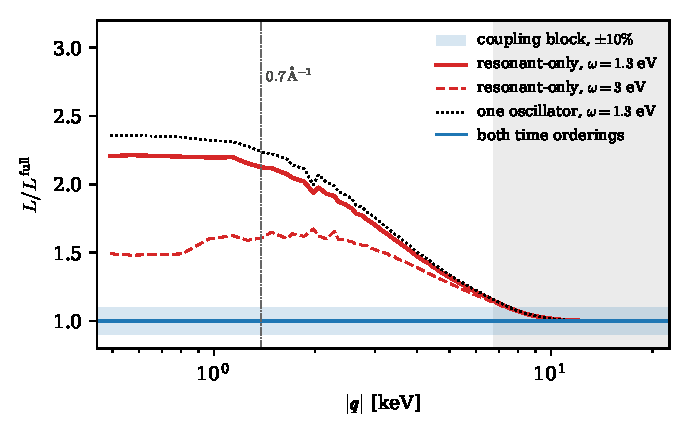
\includegraphics[width=0.82\linewidth]{figures/ch10/limit10_5a.pdf}
\captionof{figure}{Loss function of silicon in two evaluations of the same response, divided by the evaluation with both time orderings, against $|\vect{q}|$. Red: resonant-only real part, \cref{eq:10.5-kk}, at $\omega = \SI{1.3}{eV}$ (solid) and \SI{3}{eV} (dashed), from $\varepsilon_2$ of the random-phase tables with local fields of \cref{sec:10.2} (threshold \SI{1.11}{eV}, the step-model gap that accompanies them; directions averaged in bins of \SI{100}{eV}). Dotted: a single oscillator with the valence $f$-sum and the tabulated static $\varepsilon(q,0)$, \cref{eq:10.5-res}, at \SI{1.3}{eV}. Blue line and band: both time orderings, with the estimated $\pm\SI{10}{\percent}$ error of the coupling block, \cref{eq:10.5-coupling}. Dash-dotted: $|\vect{q}| = \SI{0.7}{\angstrom^{-1}}$ (\SI{1.39}{keV}), the momentum of the numbers quoted in the text. Gray: momenta at which the resonant-only form is within \SI{15}{\percent}, $|\vect{q}| \ge \SI{6.7}{keV}$.}\label{fig:10-bse-limit}
\par}
\smallskip
Below about \SI{7}{keV}, where screening is strong, a resonant-only real part overstates the loss function by up to a factor of two or more; with both time orderings the remaining error is that of the coupling block.
\end{limitbox}

\subsection{Triplet excitons}\label{sec:10.5-triplet}

A coupling to the electron spin, such as $\mathcal{O}_4$ of \cref{tab:8-operators}, creates the electron--hole pair with its spins combined to one, a triplet, and the triplet rows of \cref{tab:10-minimal} are its responses. Without interaction they are a quarter of the density response (\cref{eq:D.30-quarter}), and they are not screened (\cref{sec:10.4}). With the interaction the triplet pair has its own Bethe--Salpeter equation. The exchange kernel comes from a pair that annihilates and is re-created, and a spin-one pair cannot annihilate into the spinless density that the Coulomb line couples to, so its contribution cancels between the two spin projections. The direct kernel, the attraction between the electron and the hole, acts in every spin state alike. The triplet Hamiltonian is therefore
\begin{equation}
  H^{\mathrm{exc}}_{\mathrm{T}} = \Delta - K^{\mathrm{d}} ,
  \label{eq:10.5-triplet}
\end{equation}
\cref{eq:4.9-bse} with $g_{\mathrm{deg}}K^{\mathrm{x}}$ removed, and the spin structure factor follows from its eigenpairs as the density one does, with the vertex $\sigma^z/2$ in place of one and no $1/|\varepsilon_{\mathrm{mac}}|^2$.

The bound lines of the triplet sit where the singlet ones do, up to the electron--hole exchange splitting. That splitting is the short-range exchange of a pair whose electron and hole meet in one cell with probability of order $(a/a_x)^3$, $2\times10^{-3}$ in silicon, so it is a fraction of order $10^{-3}$ of the binding, well below a meV. And the Wannier analysis above, which used only $K^{\mathrm{d}}$, applies unchanged: the triplet edge has the same lines, the same Fermi factor and the same selection rules of point symmetry as the singlet one, with the spin vertex in place of the density vertex. What separates the two channels is the rest of $K^{\mathrm{x}}$, the local fields, which raise the singlet transitions and move weight up (\cref{sec:4.6}) and which the triplet lacks. In the model of \cref{fig:10-xq}, the triplet spectrum below \SI{3}{eV} carries 2.2 times the independent-pair weight, and between 2.5 and \SI{4}{eV} five times, while above \SI{4}{eV} the two agree within 4 percent. The attraction alone moves the triplet weight down more than the singlet's, since no local fields push back.

What is not known is the triplet response at keV momentum transfers beyond independent particles: the ladder with the screened attraction over the whole spectrum, together with the exchange--correlation kernel of the spin channel, which is not the one of the density. As an estimate, near the edge the spin rows of \cref{tab:10-minimal} inherit the excitonic enhancement of the singlet ones, without their local fields and without screening. \Cref{app:E.16} specifies the calculation, as the Bethe--Salpeter run of \cref{app:E.15} with the exchange kernel switched off; its control is the limit without interaction, which must return a quarter of the independent-particle density response.

\subsection{Open problems}\label{sec:10.5-open}

For silicon and germanium no finite-momentum Bethe--Salpeter calculation exists, with or without the coupling block, and no calculation resolves the bound lines of an indirect gap. The lines need grids around the pair minimum far finer than a uniform grid can afford, and are therefore to be added from \cref{eq:10.5-lines,eq:10.5-second} with computed masses, vertices and vertex gradients. The full coupled calculation would settle the \SI{10}{\percent} of \cref{eq:10.5-coupling}, test the factor of two of \cref{eq:10.5-res} directly, and check the $f$-sum rule to a percent (\cref{app:E.15}). The triplet response beyond independent particles is open as stated above.

So is the response of crystals in which the exciton is not large. In NaI the lowest excitons are compact, of the size of an ion pair, and the hole localizes on two anions while the lattice relaxes around it: the exciton becomes self-trapped. The Wannier picture fails, and the line that dark matter creates is dressed by the phonons that the relaxation emits. Take linear coupling, a harmonic lattice and a vertex independent of the lattice coordinates. The line at $E_\lambda$ then becomes a Poisson series of replicas spaced by a mean phonon energy $\bar\omega$, with the weight $\ee^{-S_{\mathrm{HR}}}S_{\mathrm{HR}}^n/n!$ in the $n$th (\cref{eq:E.15-ste}), where the Huang--Rhys factor $S_{\mathrm{HR}}$ is the mean number of phonons emitted, the relaxation energy divided by $\bar\omega$. For NaI none of $S_{\mathrm{HR}}$, $\bar\omega$ or the form factor $\rho_{\lambda0}(\vect{q})$ is known at keV momenta, and \cref{app:E.15} specifies their calculation. The localized (Frenkel) exciton itself, the limit of a pair confined to one site, is made precise in \cref{sec:16.4}. The spread between the random-phase and the excitonic rate near the gap, the factor that a resonant-only evaluation can introduce, and the coupling error enter the many-body uncertainty of \cref{sec:8.8}, collected for this chapter in \cref{sec:10.10}.
